% vim: set textwidth=78 autoindent:

\subsection{L'extension G\'eor\'ef\'erencer}

% when the revision of a section has been finalized, 
% comment out the following line:
% \updatedisclaimer

% The \toolbtntwo{georeferencer}{Georeferencer} allows to generate world files for rasters.
% Therefore you select points on the raster, add their coordinates, and the plugin will compute the world file parameters.
% The more coordinates you provide the better the result will be.

Le \toolbtntwo{G\'eor\'ef\'erencer}{G\'eor\'ef\'erencer} permet de g\'en\'erer un fichier world file pour les rasters (ce fichier contient toutes les informations n\'ecessaires au positionnement spatial).
Il faut pour cela, s\'electionner des points du raster et leur associer des coordonn\'ees; l'extension calculera les param\`etres du fichier world file.
Plus grand sera le nombre de coordonn\'ees fournies, meilleur sera le r\'esultat.

% As an example we will generate a world file for a topo sheet of South Dakota from SDGS.
% It can later be visualized together with in the data of the GRASS spearfish60 location.
% You can download the topo sheet here: \url{http://grass.osgeo.org/sampledata/spearfish\_toposheet.tar.gz}

En guise d'exemple, nous g\'en\'ererons un fichier world file pour une carte topographique du Dakota du Sud publi\'ee par le SDGS.
Elle pourra, par la suite, \^etre affich\'ee avec les donn\'ees du secteur GRASS spearfish60.
La carte topographique peut \^etre t\'el\'echarg\'ee \`a l'adresse suivante : \url{http://grass.osgeo.org/sampledata/spearfish\_toposheet.tar.gz}

% As a first step we download the file and untar it.

La premi\`ere \'etape est le t\'el\'echargement de ce fichier et son extraction.

\begin{verbatim}
wget http://grass.osgeo.org/sampledata/spearfish_toposheet.tar.gz
tar xvzf spearfish_toposheet.tar.gz
cd spearfish_toposheet
\end{verbatim}

% The next step is to start QGIS, load the georeferencer plugin and select the file \filename{spearfish\_topo24.tif}.

L'\'etape suivante consiste \`a d\'emarrer QGIS, charger l'extension G\'eor\'ef\'erencer et s\'electionner le fichier \filename{spearfish\_topo24.tif}.

% \begin{figure}[ht]
% \begin{center}
% \caption{Select an image to georeference \nixcaption}\label{fig:select_image}\smallskip
%   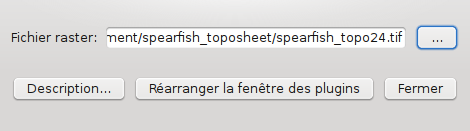
\includegraphics[clip=true, width=12cm]{select_image}
% \end{center}
% \end{figure}

\begin{figure}[ht]
\begin{center}
\caption{S\'electionner une image \`a g\'eor\'ef\'erencer \nixcaption}\label{fig:select_image}\smallskip
  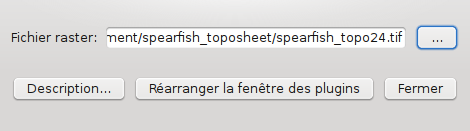
\includegraphics[clip=true, width=12cm]{select_image}
\end{center}
\end{figure}

% Now click on the button \button{Arrange plugin window} to open the image in
% the georeferencer and to arrange it with the reference map in the qgis map
% canvas on your desktop (see Figure \ref{fig:georefplugin}).

Cliquer ensuite sur le bouton \button{Arrange plugin window} pour ouvrir l'image dans
la fen\^etre de g\'eor\'ef\'erencement et pour organiser les diff\'erentes fen\^etres de QGIS sur
le bureau (voir Figure \ref{fig:georefplugin}).

% \begin{figure}[ht]
% \begin{center}
  % \caption{Arrange plugin window with the qgis map canvas \nixcaption}\label{fig:georefplugin}\smallskip
  % 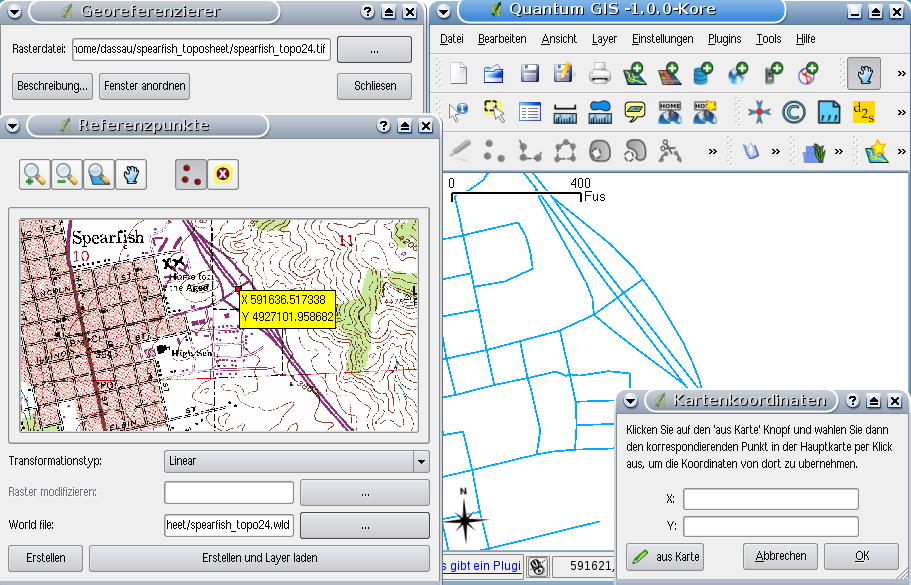
\includegraphics[clip=true,width=\textwidth]{georefplugin}
% \end{center}
% \end{figure}

\begin{figure}[ht]
\begin{center}
  \caption{Organiser les fen\^etres de QGIS sur le bureau \nixcaption}\label{fig:georefplugin}\smallskip
  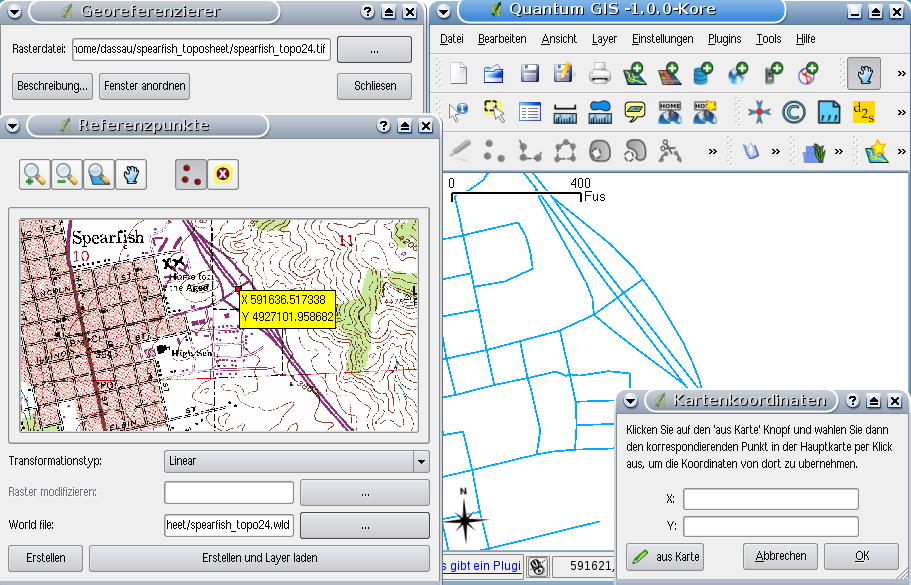
\includegraphics[clip=true,width=\textwidth]{georefplugin}
\end{center}
\end{figure}

% With the button \button{Add Point} you can start to add points on the raster image and enter their coordinates, and the plugin will compute the world file parameters (see Figure \ref{fig:choose_points}).
% The more coordinates you provide the better the result will be.
% For the procedure you have two options:

Avec le bouton \button{Add Point} on peut commencer \`a ajouter des points sur l'image raster et entrer leurs coordonn\'ees. L'extension calculera les param\`etres du fichier world file (voir Figure \ref{fig:choose_points}).
Plus on fournit de coordonn\'ees, meilleur sera le r\'esultat.
Il y a deux mani\`eres de proc\'eder :

% \begin{enumerate}
% \item You click on a point in the raster map and enter the X and Y coordinates manually
% \item You click on a point in the raster map and choose the button \button{from map canvas} to add the X and Y coordinates with the help of a georeferenced map already loaded in QGIS.
% \end{enumerate}

\begin{enumerate}
\item Cliquer en un point de la carte raster et entrer les coordonn\'ees X et Y manuellement
\item Cliquer en un point de la carte raster puis sur le bouton \button{from map canvas} pour ajouter les coordonn\'ees X et Y \`a l'aide d'une carte g\'eor\'ef\'erenc\'ee d\'ej\`a charg\'ee dans QGIS.
\end{enumerate}

% \begin{figure}[ht]
% \begin{center}
  % \caption{Add points to the raster image \nixcaption}\label{fig:choose_points}\smallskip
  % 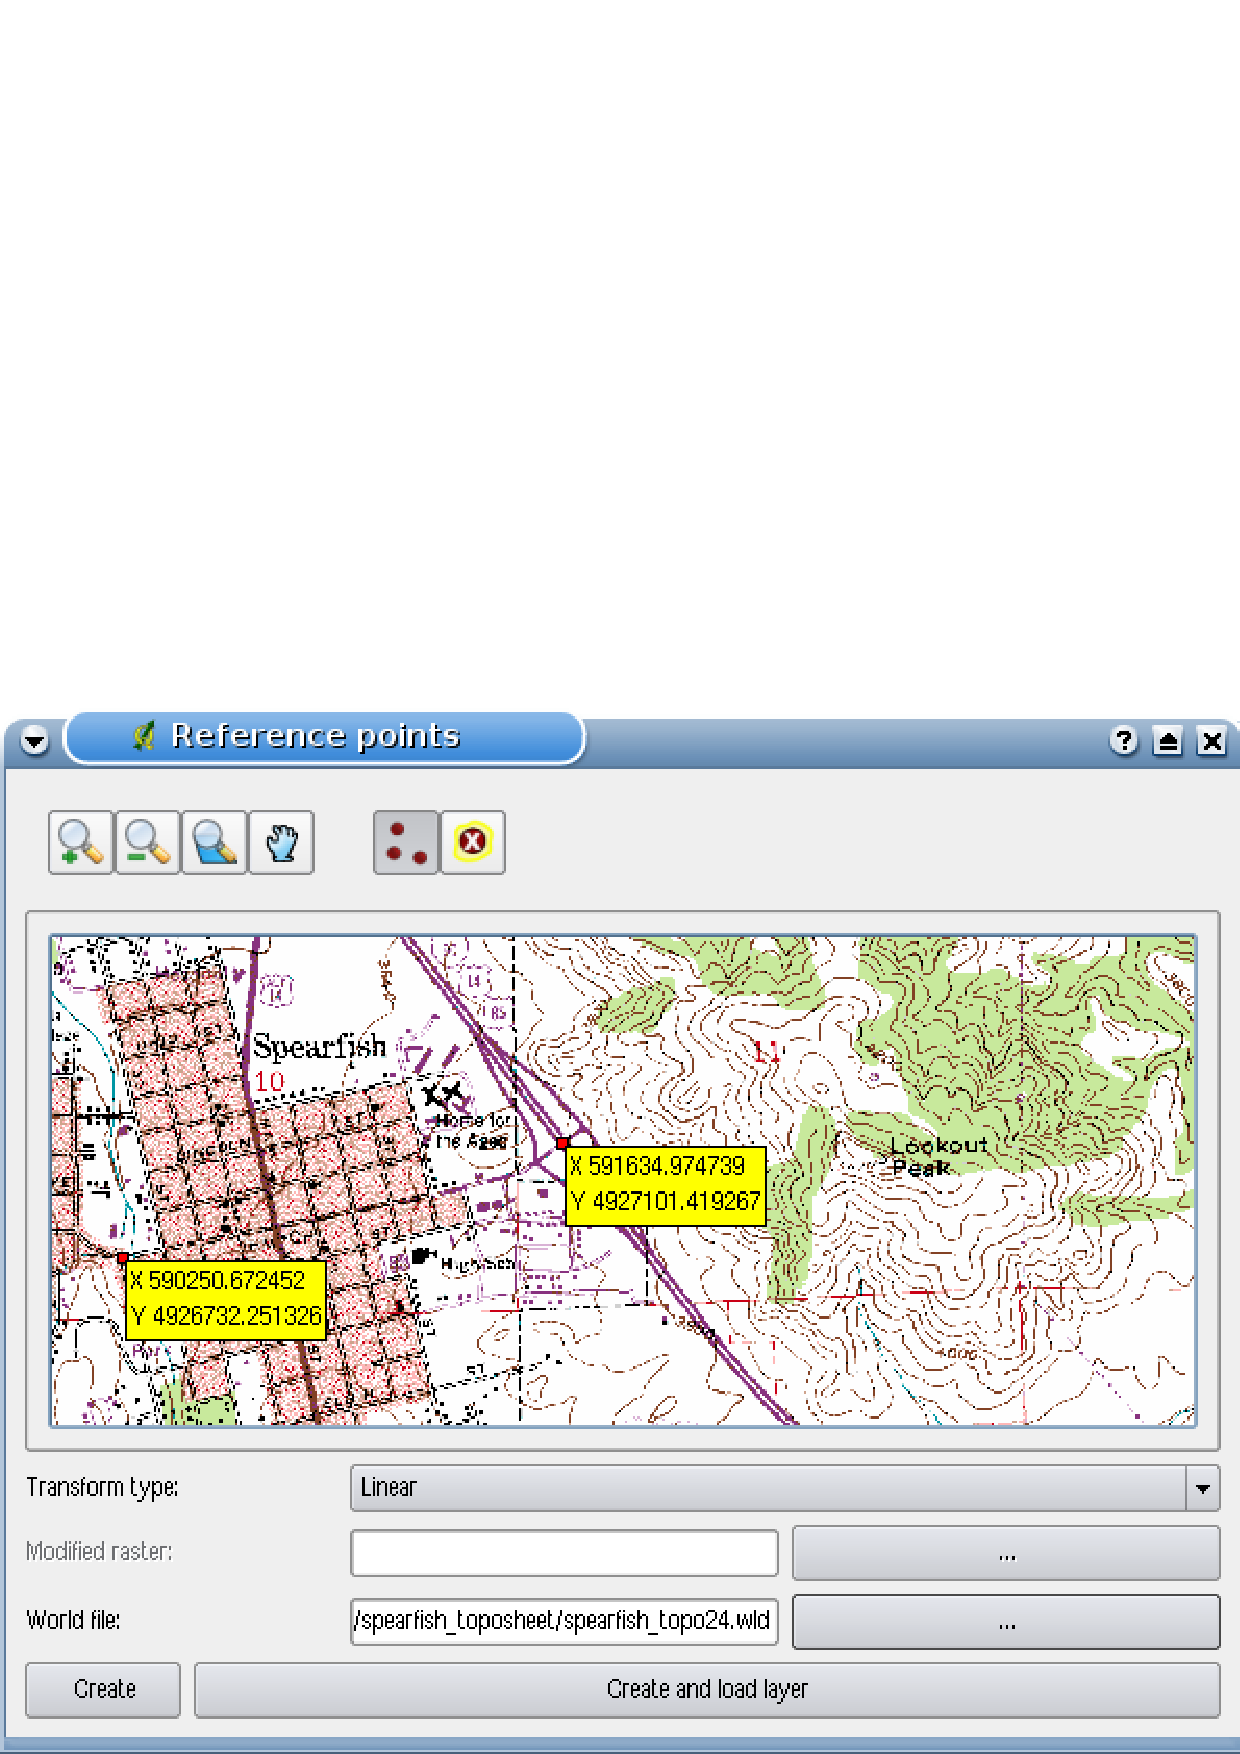
\includegraphics[clip=true,width=0.9\textwidth]{choose_points}
% \end{center}
% \end{figure}

\begin{figure}[ht]
\begin{center}
  \caption{Ajouter les points \`a l'image raster \nixcaption}\label{fig:choose_points}\smallskip
  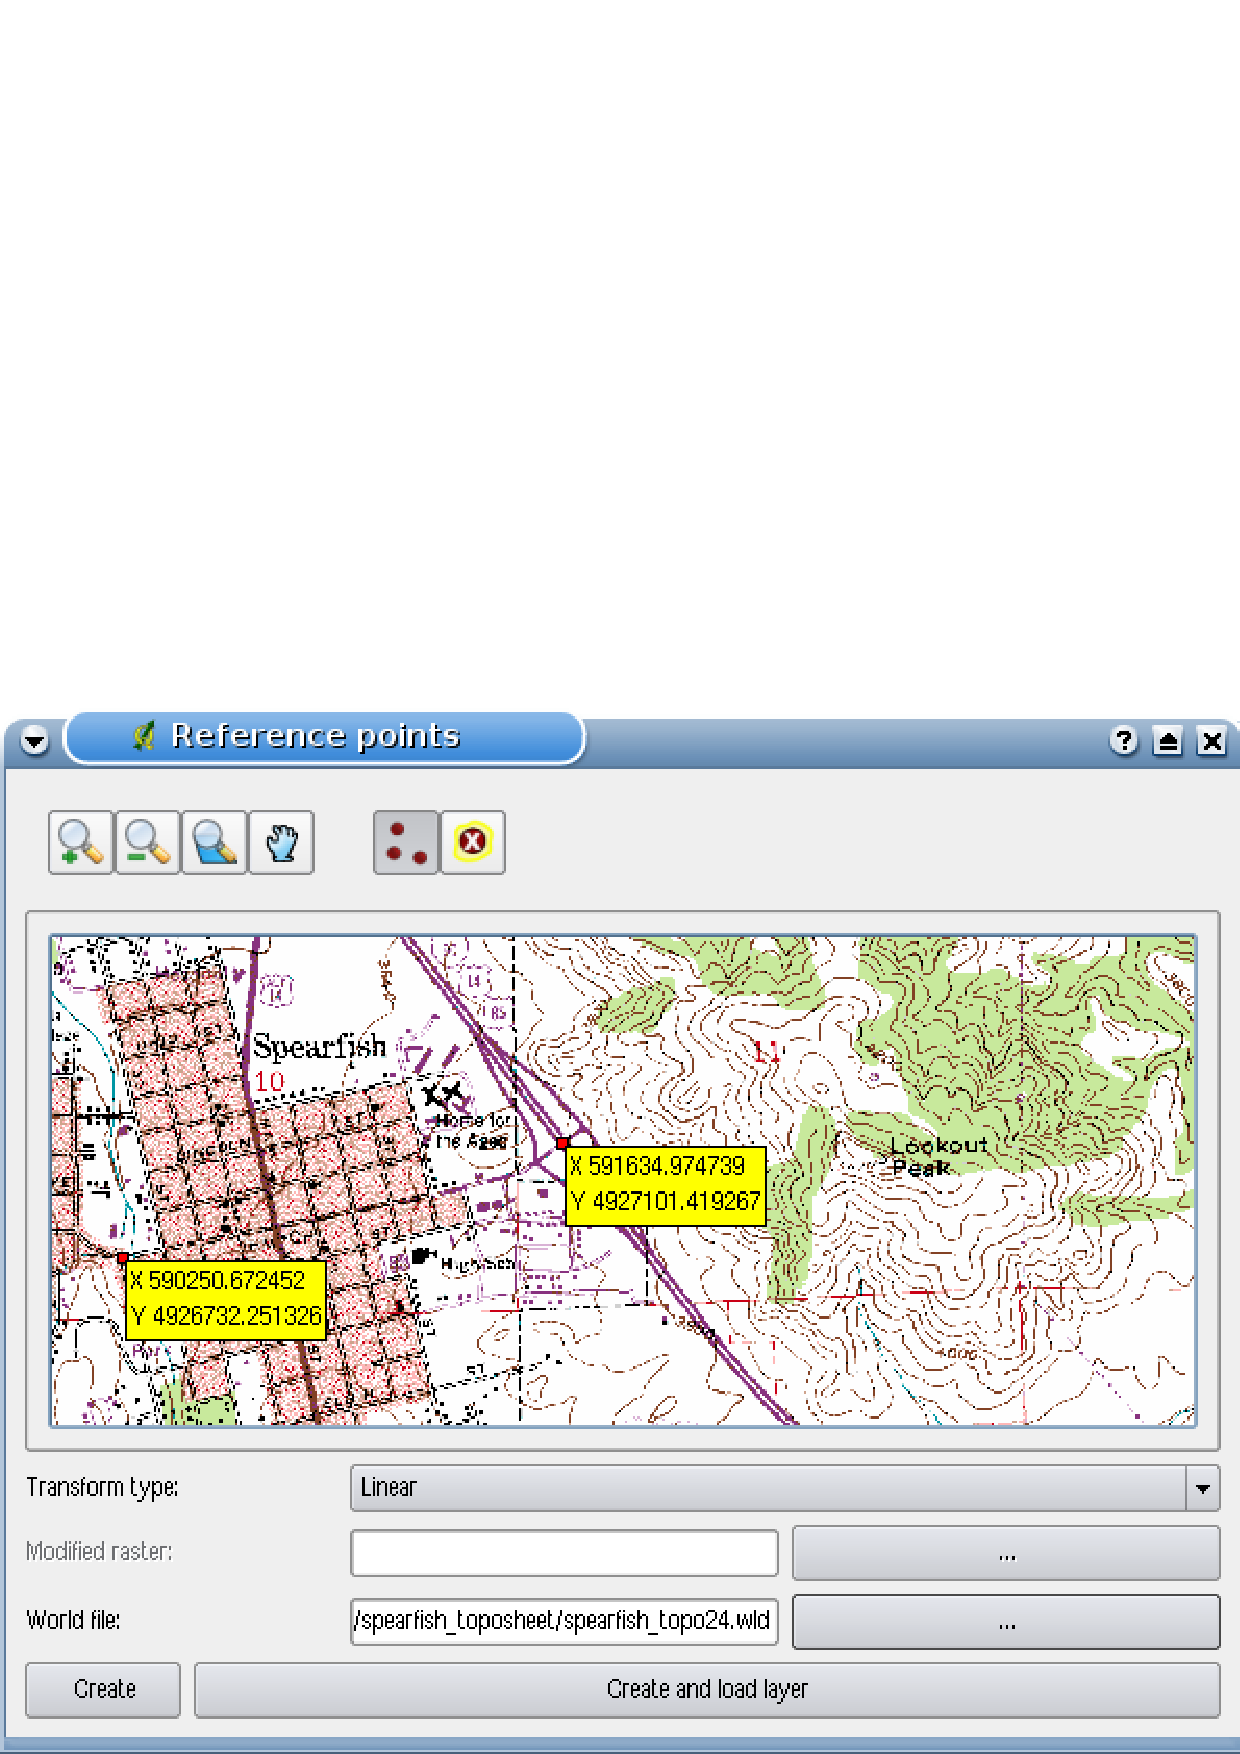
\includegraphics[clip=true,width=0.9\textwidth]{choose_points}
\end{center}
\end{figure}

% For this example we use the second option and enter the coordinates for the selected points with the help of the \filename{roads} map provided with the  \filename{spearfish60} location from: \url{http://grass.osgeo.org/sampledata/spearfish\_grass60data-0.3.tar.gz}

Pour cet exemple, nous utilisons la seconde proc\'edure et entrons les coordonn\'ees des points s\'electionn\'es \`a l'aide de la carte \filename{roads} fournie avec le secteur \filename{spearfish60} disponible \`a l'adresse suivante : \url{http://grass.osgeo.org/sampledata/spearfish\_grass60data-0.3.tar.gz}

% If you don't know how to integrate the \filename{spearfish60} location with
% the GRASS plugin, information are provided in Section \ref{sec:grass}. As you
% can see in Figure \ref{fig:choose_points}, the georeferencer provides buttons to zoom, pan, add and delete points in the image.

Si vous ne savez pas comment int\'egrer le secteur \filename{spearfish60} avec
l'extension GRASS, des explications sont disponibles dans la section \ref{sec:grass}. Comme on
peut le voir dans la Figure \ref{fig:choose_points}, l'outil de g\'eor\'ef\'erencement dispose de boutons pour le changement d'\'echelle, la translation, l'ajout et la suppression de points dans l'image.

% After you added enough points to the image you need to select the transformation type for the georeferencing process and save the resulting world file together with the Tiff.
% In our example we choose 
% \selectstring{Transform type}{linear transformation} 
% although a 
% \selectstring{Transform type}{Helmert transformation}
% might be sufficient as well.

Apr\`es avoir ajouter suffisamment de points \`a l'image, on peut s\'electionner le type de transformation pour le processus de g\'eor\'ef\'erencement et sauver le fichier world file avec le fichier Tiff.
Dans notre exemple, nous avons choisi
\selectstring{Transform type}{linear transformation}
bien que
\selectstring{Transform type}{Helmert transformation}
pourrait tout aussi bien convenir.

% \begin{Tip}\caption{\textsc{Choosing the transformation type}}
% \qgistip{The linear (affine) transformation is a 1st order transformation and is used for scaling, translation and rotation of geometrically correct images.
% With the Helmert transformation you simply add coordinate information to the image like geocooding.
% If your image is contorted you will need to use software that provides 2nd or 3rd order polynomial transformation, e.g. GRASS GIS.}
% \end{Tip} 

\begin{Tip}\caption{\textsc{Choisir le type de transformation}}
\qgistip{La transformation lin\'eaire (affine) est une tranformation de 1er ordre et est utilis\'ee pour la mise \`a l'\'echelle, la translation et la rotation d'images g\'eom\'etriquement correctes.
Avec la transfomation de Helmert, on ajoute simplement des informations de type g\'eocodage \`a l'image.
Si l'image est distordue, il sera n\'ecessaire d'utiliser une logiciel permettant les transformations polynomiales de 2nd et 3\`eme ordre, comme GRASS GIS par exemple}
\end{Tip} 

% The points we added to the map will be stored in a \filename{spearfish\_topo24.tif.points} file together with the raster image.
% This allows us to reopen the georeferencer plugin and to add new points or delete existing ones to optimize the result.
% The \filename{spearfish\_topo24.tif.points} file of this example shows the points:

Les points ajout\'es \`a la carte seront conserv\'es dans un fichier \filename{spearfish\_topo24.tif.points} adjoint \`a l'image raster.
Ceci permet d'optimiser le r\'esultat en ouvrant de nouveau l'extension G\'eor\'ef\'erencer et en ajoutant de nouveaux points ou supprimant des points existants.
Le fichier \filename{spearfish\_topo24.tif.points} de cet exemple contient les points suivants :

\begin{verbatim}
mapX    		mapY    		pixelX  pixelY
591630.196867999969982  4927104.309682800434530 591647  4.9271e+06
608453.589164100005291  4924878.995150799863040 608458  4.92487e+06
602554.903929700027220  4915579.220743400044739 602549  4.91556e+06
591511.138448899961077  4915952.302661700174212 591563  4.91593e+06
602649.526155399973504  4919088.353569299913943 602618  4.91907e+06
\end{verbatim} 

% We used 5 coordinate points to georeference the raster image.
% To get correct results it is important to disperse the points regulary in the image.
% Finally we check the result and load the new georeferenced map \filename{spearfish\_topo24.tif} and overlay it with the map \filename{roads} of the \filename{spearfish60} location.

Cinq points ont \'et\'e utilis\'es pour g\'eor\'ef\'erencer l'image raster.
Pour obtenir des r\'esultats corrects, il est important de r\'epartir les points r\'eguli\`erement sur l'image.
Finalement on peut v\'erifier le r\'esultat, charger la nouvelle carte g\'eor\'ef\'erenc\'ee \filename{spearfish\_topo24.tif} et la superposer \`a la carte \filename{roads} du secteur \filename{spearfish60}.

% \begin{figure}[ht]
% \begin{center}
  % \caption{Georeferenced map with overlayed roads from spearfish60 location
  % \nixcaption}\label{fig:result_map}\smallskip
  % 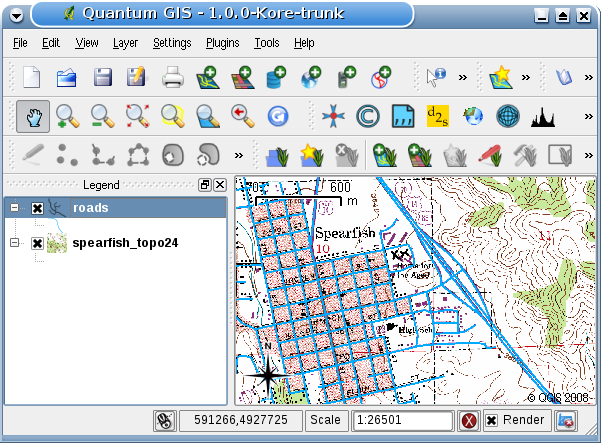
\includegraphics[clip=true,width=\textwidth]{result_map}
% \end{center}
% \end{figure}

\begin{figure}[ht]
\begin{center}
  \caption{Carte g\'eor\'ef\'erenc\'ee avec superposition des routes provenant du secteur spearfish60
  \nixcaption}\label{fig:result_map}\smallskip
  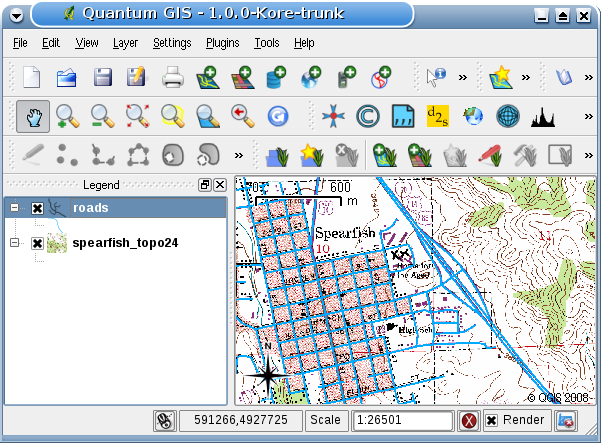
\includegraphics[clip=true,width=\textwidth]{result_map}
\end{center}
\end{figure}
